\newcommand{\zoomin}[9]{ %
\begin{tikzpicture}[spy using outlines={rectangle,#9,magnification=#8,size=#6}]   
	\node[anchor=south west,inner sep=0]  {\includegraphics[width=#7]{#1}};
	\spy on (#2, #3) in node at (#4,#5);
\end{tikzpicture}
}

\begin{figure*}[!h]
	\newlength\mytmplen
	\setlength\mytmplen{.193\linewidth}
	\setlength{\tabcolsep}{1pt}
	\renewcommand{\arraystretch}{0.5}
	\centering
	\begin{tabular}{cccccc}
		Ground Truth&Ours& Mip-NeRF360 & InstantNGP & Plenoxels \\
		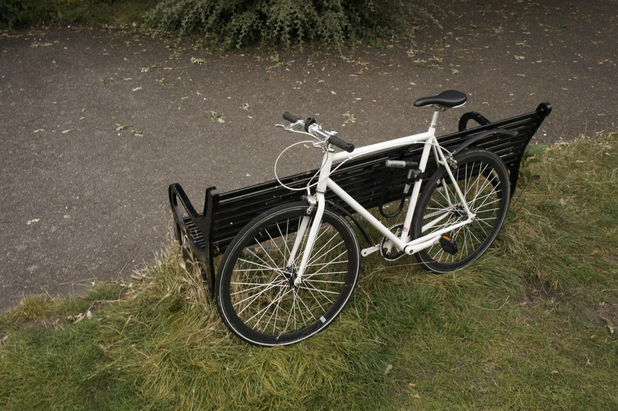
\includegraphics[width=\mytmplen,trim={0 1.5cm 0 2cm},clip]{results2/bicycle/gt/DSC8824_s.png} &
		
\includegraphics[width=\mytmplen,trim={0 1.5cm 0 2cm},clip]{results2/bicycle/ours/DSC8824_s.png} &
	    \begin{tikzpicture}
			\node[anchor=south west,inner sep=0] (image) at (0,0) {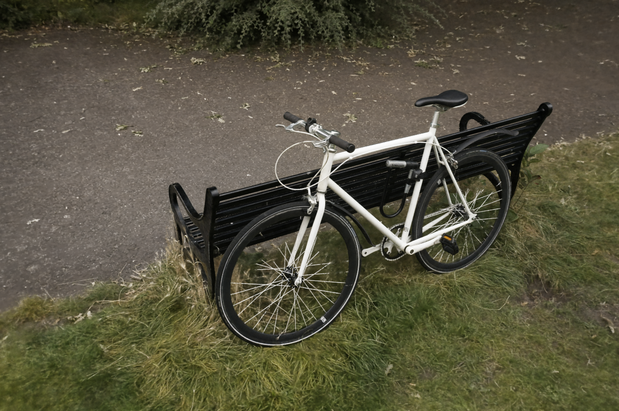
\includegraphics[width=\mytmplen,trim={0 1.5cm 0 2cm},clip]{results2/bicycle/mipnerf360/color_018_s.png}};
			\begin{scope}[x={(image.south east)},y={(image.north west)}]
				\draw[red,ultra thick,->] (0.23,0.40) -- (0.38,0.40);
			\end{scope}
		\end{tikzpicture} &
		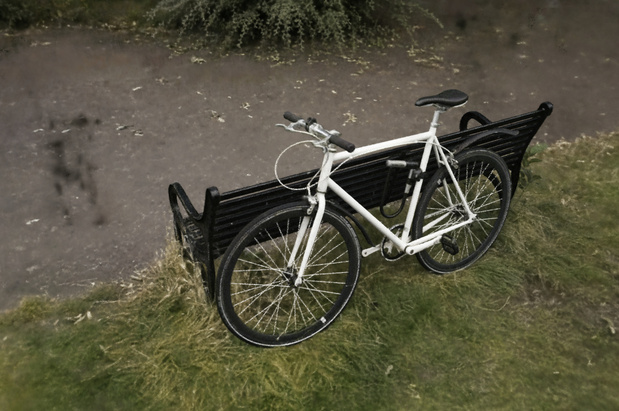
\includegraphics[width=\mytmplen,trim={0 1.5cm 0 2cm},clip]{results2/bicycle/igp/out_DSC8824_s.jpg} &
			    \begin{tikzpicture}
			\node[anchor=south west,inner sep=0] (image) at (0,0) {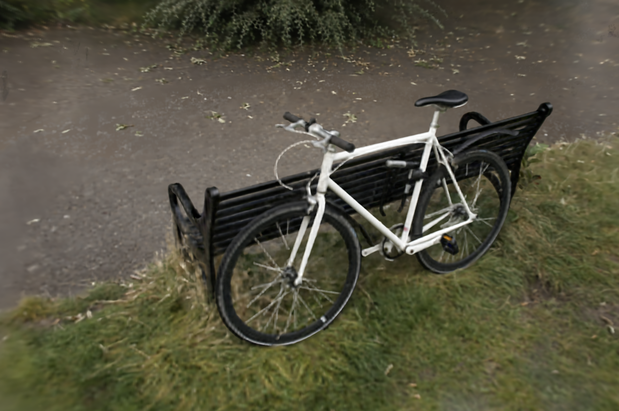
\includegraphics[width=\mytmplen,trim={0 1.5cm 0 2cm},clip]{results2/bicycle/plenoxels/render_0018_s.png}};
			\begin{scope}[x={(image.south east)},y={(image.north west)}]
				\draw[red,ultra thick,->] (0.23,0.40) -- (0.38,0.40);
			\end{scope}
		\end{tikzpicture} \\
		\zoomin{results2/garden/gt/gt_001.png}{0.6}{1.95}{0.55cm}{0.55cm}{1cm}{\mytmplen}{3}{red}&
		\zoomin{results2/garden/ours/DSC07964.png}{0.6}{1.95}{0.55cm}{0.55cm}{1cm}{\mytmplen}{3}{red}&
		\zoomin{results2/garden/mipnerf360/color_001.png}{0.6}{1.95}{0.55cm}{0.55cm}{1cm}{\mytmplen}{3}{red}&
		\zoomin{results2/garden/igp/out_DSC07964.jpg}{0.6}{1.95}{0.55cm}{0.55cm}{1cm}{\mytmplen}{3}{red}&
		\zoomin{results2/garden/plenoxels/render_0001.png}{0.6}{1.95}{0.55cm}{0.55cm}{1cm}{\mytmplen}{3}{red}\\
		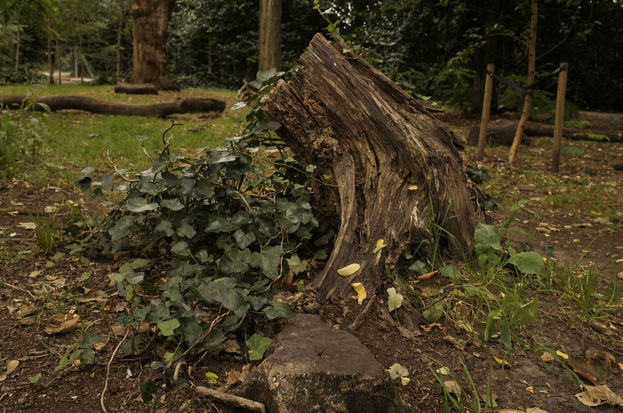
\includegraphics[width=\mytmplen]{results2/stump/gt/DSC9237_s.png} &
		
\includegraphics[width=\mytmplen]{results2/stump/ours/DSC9237_s.png} &
		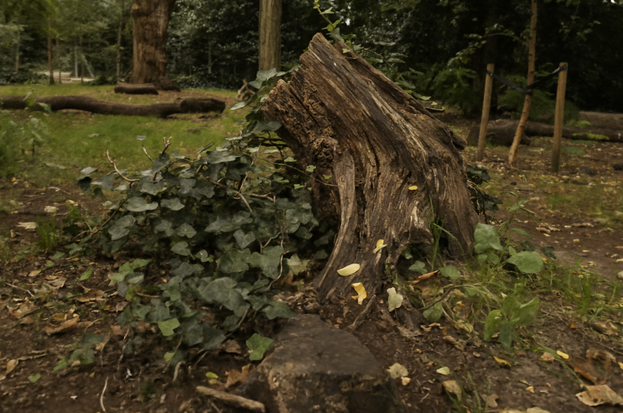
\includegraphics[width=\mytmplen]{results2/stump/mipnerf360/color_003_s.png} &
		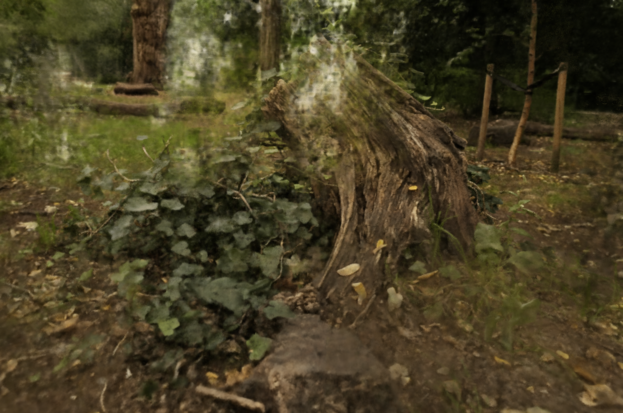
\includegraphics[width=\mytmplen]{results2/stump/igp/out_0003_s.png} &
		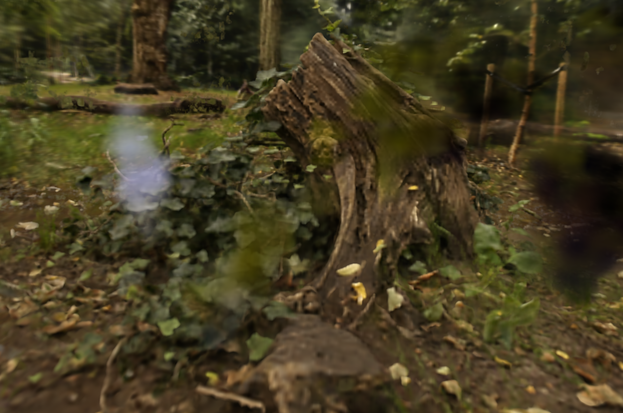
\includegraphics[width=\mytmplen]{results2/stump/plenoxels/render_0003_s.png} 
		\\
		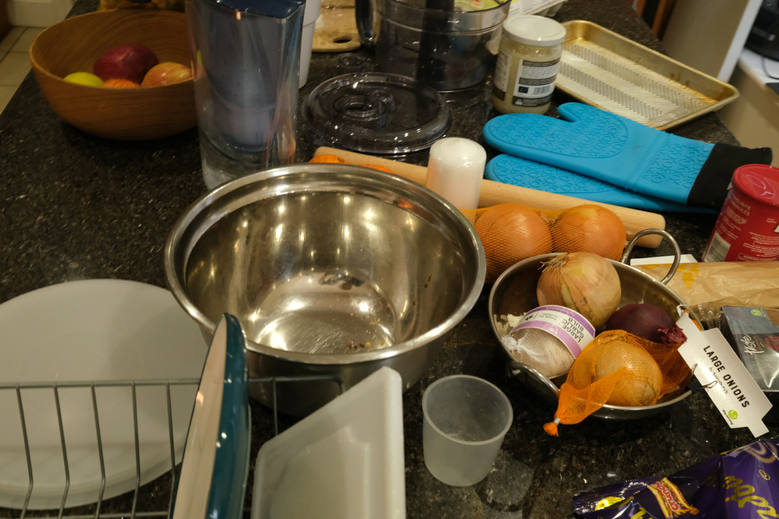
\includegraphics[width=\mytmplen]{results2/counter/gt/DSCF6089_s.png} &
		
\includegraphics[width=\mytmplen]{results2/counter/ours/DSCF6089_s.png} &
 		\begin{tikzpicture}
			\node[anchor=south west,inner sep=0] (image) at (0,0) {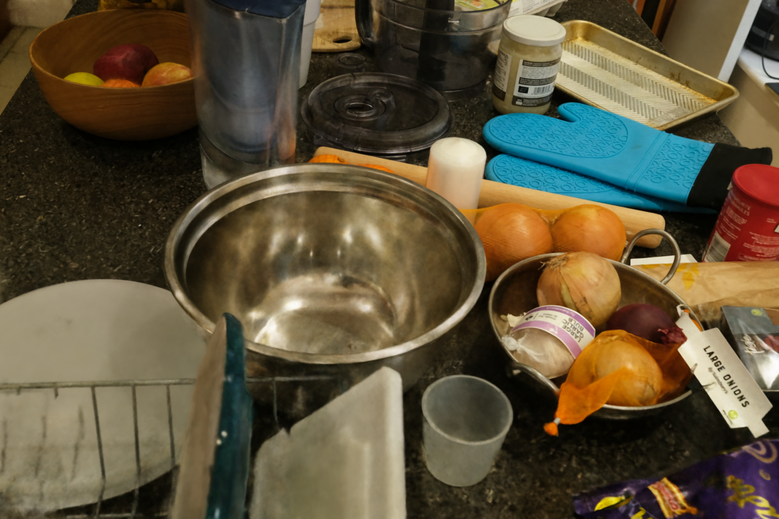
\includegraphics[width=\mytmplen]{results2/counter/mipnerf360/color_029_s.png}};
			\begin{scope}[x={(image.south east)},y={(image.north west)}]
				\draw[red,ultra thick,->] (0.07,0.43) -- (0.07,0.23);
			\end{scope}
		\end{tikzpicture} &
		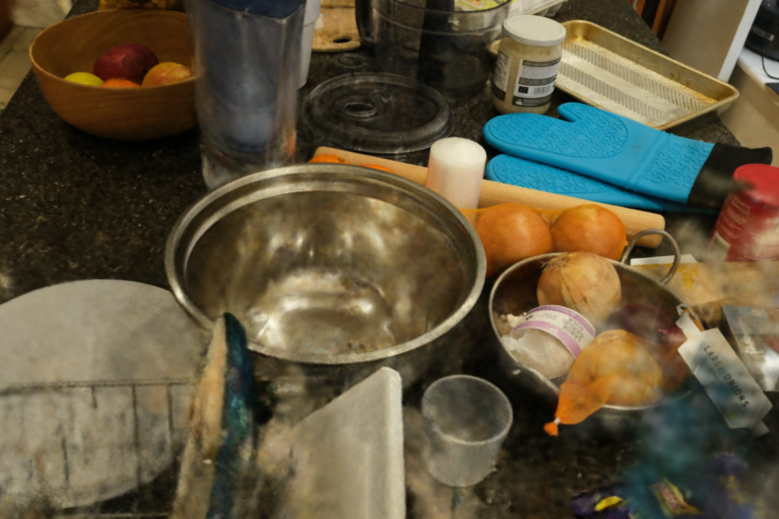
\includegraphics[width=\mytmplen]{results2/counter/igp/out_0029_s.png} &
		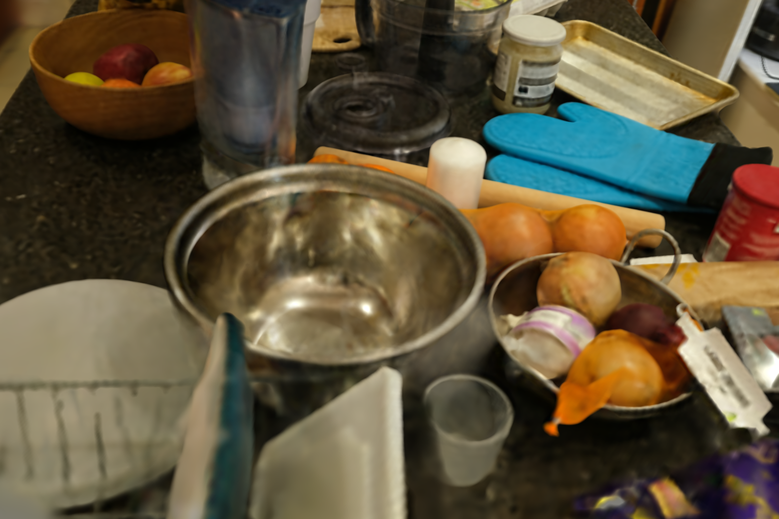
\includegraphics[width=\mytmplen]{results2/counter/plenoxels/render_0029_s.png} 
		\\
		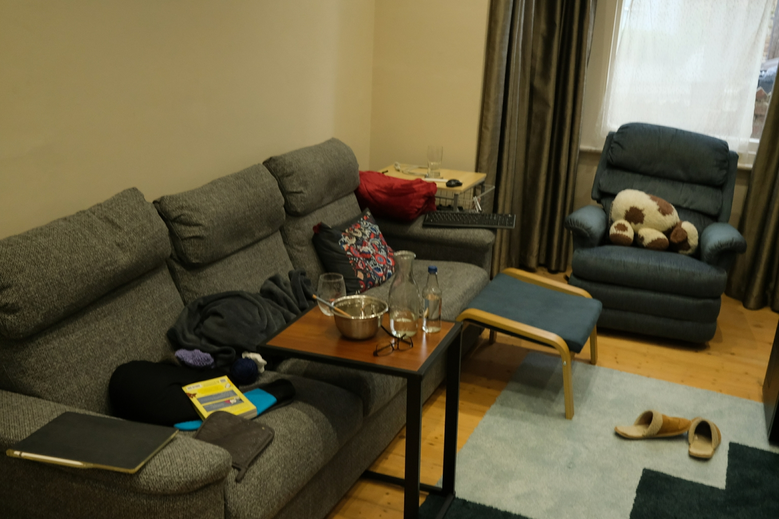
\includegraphics[width=\mytmplen]{results2/room/gt/gt_0025_s.png} &
		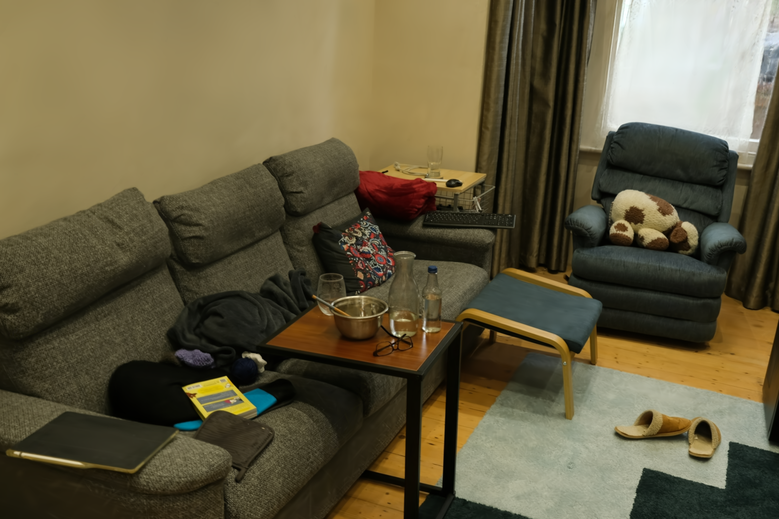
\includegraphics[width=\mytmplen]{results2/room/ours/DSCF4867_s.png} &
		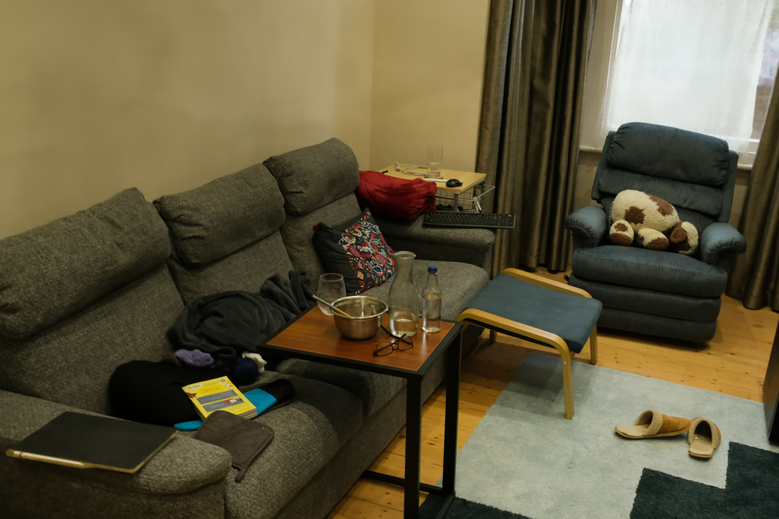
\includegraphics[width=\mytmplen]{results2/room/mipnerf360/color_025_s.png} &
		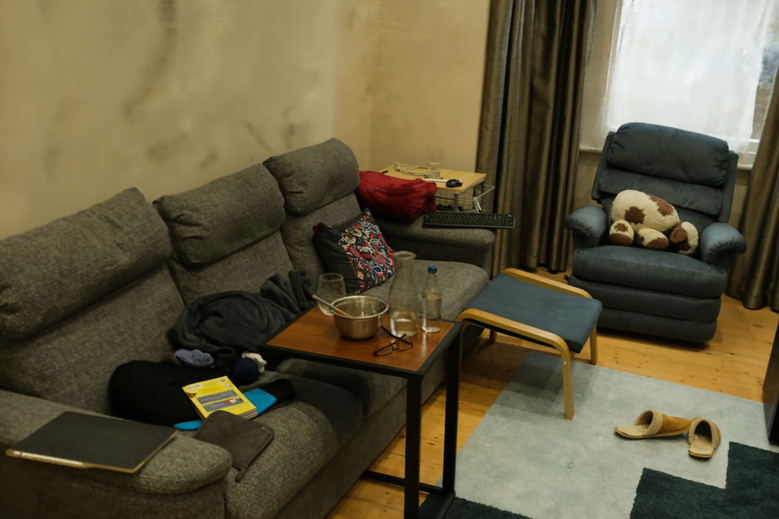
\includegraphics[width=\mytmplen]{results2/room/igp/out_DSCF4867_s.jpg} &
		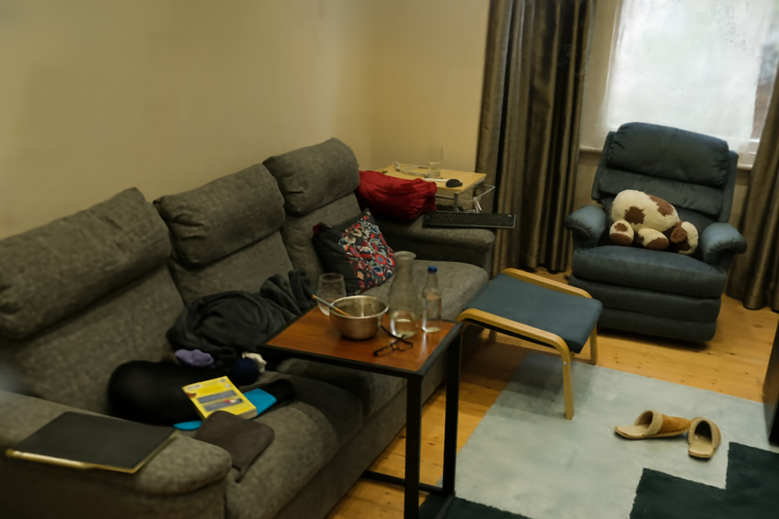
\includegraphics[width=\mytmplen]{results2/room/plenoxels/render_0025_s.png} \\
		\zoomin{results2/playroom/gt/gt_014_s.png}{1.2}{1.4}{0.55cm}{0.55cm}{1cm}{\mytmplen}{3}{green}&
		\zoomin{results2/playroom/ours/DSC05686_s.png}{1.2}{1.4}{0.55cm}{0.55cm}{1cm}{\mytmplen}{3}{green}&
		\zoomin{results2/playroom/mipnerf360/color_014_s.png}{1.2}{1.4}{0.55cm}{0.55cm}{1cm}{\mytmplen}{3}{green}&
		\zoomin{results2/playroom/igp/out_0014_s.png}{1.2}{1.4}{0.55cm}{0.55cm}{1cm}{\mytmplen}{3}{green}& 
		\zoomin{results2/playroom/plenoxels/render_0014_s.png}{1.2}{1.4}{0.55cm}{0.55cm}{1cm}{\mytmplen}{3}{green}
\\
		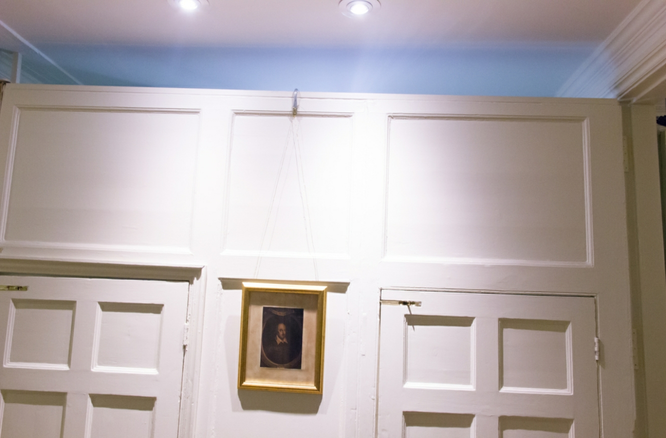
\includegraphics[width=\mytmplen]{results2/drjohnson/gt/IMG_6366_s.png} &
		
\includegraphics[width=\mytmplen]{results2/drjohnson/ours/IMG_6366_s.png} &
		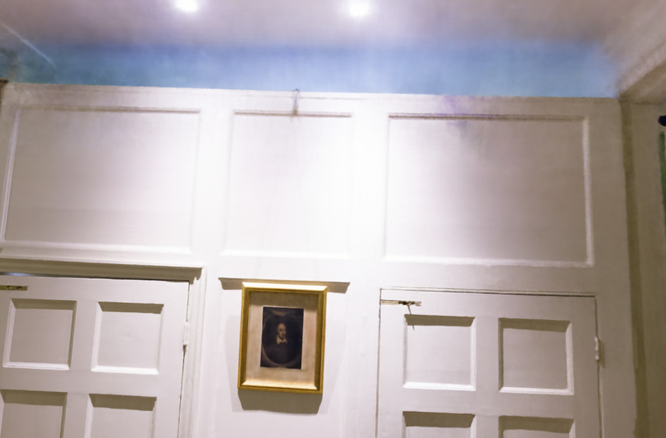
\includegraphics[width=\mytmplen]{results2/drjohnson/mipnerf360/color_008_s.png} &
		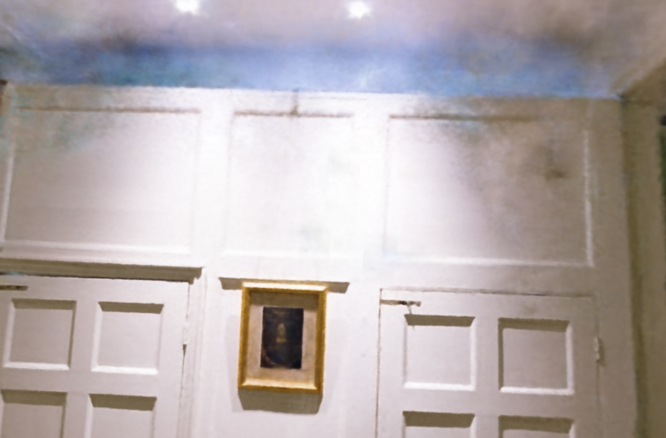
\includegraphics[width=\mytmplen]{results2/drjohnson/igp/out_0008_s.png} & 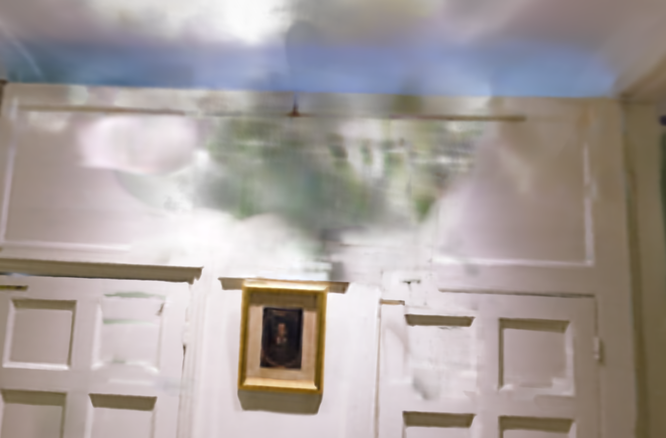
\includegraphics[width=\mytmplen]{results2/drjohnson/plenoxels/render_0008_s.png} 
\\
		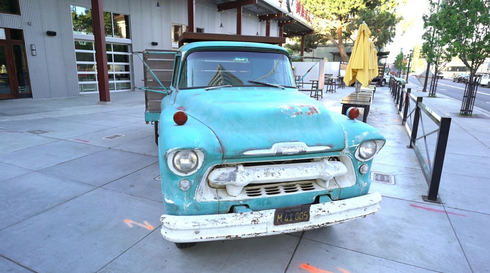
\includegraphics[width=\mytmplen]{results2/truck/gt/000065_s.png} &
		
\includegraphics[width=\mytmplen]{results2/truck/ours/000065_s.png} &
		 		\begin{tikzpicture}
			\node[anchor=south west,inner sep=0] (image) at (0,0) {
\includegraphics[width=\mytmplen]{results2/truck/mipnerf360/color_008_s.png}};
			\begin{scope}[x={(image.south east)},y={(image.north west)}]
				\draw[red,ultra thick,->] (0.87,0.11) -- (0.87,0.31);
			\end{scope}
		\end{tikzpicture} &
		
\includegraphics[width=\mytmplen]{results2/truck/igp/out_0008_s.png} &
		
\includegraphics[width=\mytmplen]{results2/truck/plenoxels/render_0008_s.png} 
\\
		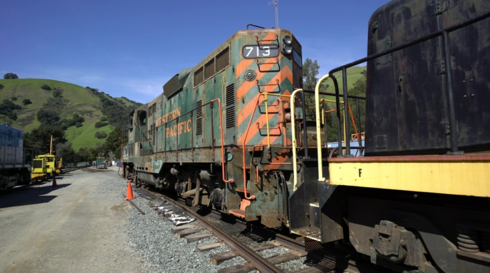
\includegraphics[width=\mytmplen]{results2/train/gt/gt_0008_s.png} &
		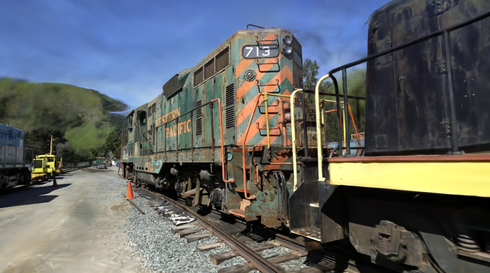
\includegraphics[width=\mytmplen]{results2/train/ours/00065_s.png} &
		
\includegraphics[width=\mytmplen]{results2/train/mipnerf360/color_008_s.png} &
		
\includegraphics[width=\mytmplen]{results2/train/igp/out_0008_s.png} &
		
\includegraphics[width=\mytmplen]{results2/train/plenoxels/render_0008_s.png} \\
	\end{tabular}
    \vspace{-.3cm} %
	\caption{
		\label{fig:comparisons}
		We show comparisons of ours to previous methods and the corresponding ground truth images from \CORRECTION{paths not in the input views}{held-out test views}. The scenes are, from the top down:
		\textsc{Bicycle}, \textsc{Garden}, \textsc{Stump}, \textsc{Counter} and \textsc{Room} from the Mip-NeRF360 dataset; \textsc{Playroom}, \textsc{DrJohnson} from the Deep Blending dataset~\cite{hedman2018deep} and \textsc{Truck} and \textsc{Train} from Tanks\&Temples. \ADDITION{Non-obvious differences in quality highlighted by arrows/insets.}
	}
\end{figure*}

\begin{table*}[!h]
	\caption{
		\label{tab:comparisons} {\CORRECTION{Quantitative evaluation of our method compared to previous work, computed over our five scenes, on separate paths captured specifically for evaluation, and separate from the input views.}{Quantitative evaluation of our method compared to previous work, computed over three datasets. Results marked with dagger $\dagger$ have been directly adopted from the original paper, all others were obtained in our own experiments.}}
	}
	\small
	\scalebox{0.78}{
		\begin{tabular}{l|cccccc|cccccc|cccccc}
			
			Dataset & \multicolumn{6}{c|}{Mip-NeRF360}  & \multicolumn{6}{c|}{Tanks\&Temples} & \multicolumn{6}{c}{Deep Blending}\\
			Method|Metric
			& $SSIM^\uparrow$   & $PSNR^\uparrow$    & $LPIPS^\downarrow$  & Train & FPS & Mem 
			& $SSIM^\uparrow$   & $PSNR^\uparrow$    & $LPIPS^\downarrow$  & Train & FPS & Mem 
			& $SSIM^\uparrow$   & $PSNR^\uparrow$    & $LPIPS^\downarrow$  & Train & FPS & Mem \\
			\hline 
			Plenoxels& 0.626 & 23.08 & 0.463 & 25m49s & 6.79 & 2.1GB & 0.719 & 21.08 & 0.379 & 25m5s & 13.0 & 2.3GB & 0.795 & 23.06 & 0.510 & 27m49s & 11.2 & 2.7GB \\
			INGP-Base& 0.671 & 25.30 & 0.371 & 5m37s & 11.7 & 13MB & 0.723 & 21.72 & 0.330 & 5m26s & 17.1 & 13MB & 0.797 & 23.62 & 0.423 & 6m31s & 3.26 & 13MB \\ 
			INGP-Big& 0.699 & 25.59 & 0.331 & 7m30s & 9.43 & 48MB & 0.745 & \cellcolor{yellow!40}21.92 & 0.305 & 6m59s & 14.4 & 48MB & 0.817 & 24.96 & 0.390 & 8m & 2.79 & 48MB \\ 
			M-NeRF360&\cellcolor{orange!40}0.792$^\dagger$ & \cellcolor{red!40} 27.69$^\dagger$ & \cellcolor{orange!40}0.237$^\dagger$ & 48h & 0.06 & 8.6MB  & \cellcolor{yellow!40}0.759 & \cellcolor{orange!40}22.22 & \cellcolor{orange!40}0.257 & 48h & 0.14 & 8.6MB & \cellcolor{orange!40}0.901 & \cellcolor{orange!40}29.40 &  \cellcolor{orange!40}0.245 & 48h & 0.09 & 8.6MB\\
			Ours-7K& \cellcolor{yellow!40}0.770 & \cellcolor{yellow!40}25.60 & \cellcolor{yellow!40}0.279 & 6m25s & 160 & 523MB & \cellcolor{orange!40}0.767 & 21.20 & \cellcolor{yellow!40}0.280 & 6m55s & 197 & 270MB & \cellcolor{yellow!40}0.875 &\cellcolor{yellow!40}27.78 & \cellcolor{yellow!40}0.317 & 4m35s & 172 & 386MB \\
			Ours-30K& \cellcolor{red!40}0.815 &  \cellcolor{orange!40}27.21 & \cellcolor{red!40}0.214 & 41m33s & 134 & 734MB & \cellcolor{red!40}0.841 & \cellcolor{red!40}23.14 & \cellcolor{red!40}0.183 & 26m54s & 154 & 411MB & \cellcolor{red!40}0.903 & \cellcolor{red!40}29.41 & \cellcolor{red!40}0.243 & 36m2s & 137 & 676MB\\
			
		\end{tabular}
	}
\end{table*}

\begin{figure}[h]
	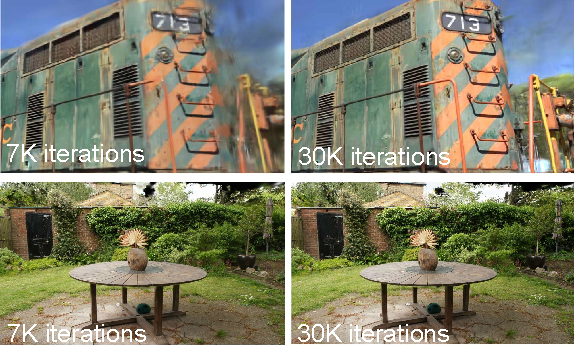
\includegraphics[width=\linewidth]{figures/ablations/7K_vs_30K.pdf} 
	\caption{
		\label{fig:5vs40min}
		For some scenes (above) we can see that even at 7K iterations ($\sim$5min for this scene), our method has captured the train quite well. At 30K iterations ($\sim$35min) the background artifacts have been reduced significantly. For other scenes (below), the difference is barely visible; 7K iterations ($\sim$8min) is already very high quality.
	}
\end{figure}

\section{Implementation, results and evaluation}

We next discuss some details of implementation, present results and the evaluation of our algorithm compared to previous work and ablation studies.

\begin{table}[!h]
	\caption{PSNR scores for Synthetic NeRF, we start with 100K randomly initialized points. \ADDITION{Competing} metrics extracted from respective papers. }
	\scalebox{0.7}{
		\centering
		\begin{tabular}{l|ccccccccc}
			~ & Mic & Chair & Ship & Materials & Lego & Drums & Ficus & Hotdog & Avg.  \\ \hline
			Plenoxels & 33.26 & 33.98 & 29.62 & 29.14 & 34.10 & 25.35 & 31.83 & 36.81 & 31.76  \\
			INGP-Base & \cellcolor{orange!40}36.22 & 35.00 & \cellcolor{red!40}31.10 & \cellcolor{yellow!40}29.78 & \cellcolor{red!40}36.39 & \cellcolor{yellow!40}26.02 & \cellcolor{yellow!40}33.51 & \cellcolor{yellow!40}37.40 & \cellcolor{yellow!40}33.18  \\ 
			Mip-NeRF & \cellcolor{red!40}36.51 & \cellcolor{yellow!40}35.14 & 30.41 & \cellcolor{red!40}30.71 & \cellcolor{yellow!40}35.70 & 25.48 & 33.29 & \cellcolor{orange!40}37.48 & 33.09  \\ 
			Point-NeRF & \cellcolor{yellow!40}35.95 & \cellcolor{orange!40}35.40 & \cellcolor{orange!40}30.97 & 29.61 & 35.04 & \cellcolor{orange!40}26.06 & \cellcolor{red!40}36.13 & 37.30 & \cellcolor{orange!40}33.30  \\  
			Ours-30K & 35.36 & \cellcolor{red!40}35.83 & \cellcolor{yellow!40}30.80 & \cellcolor{orange!40}30.00 & \cellcolor{orange!40}35.78 & \cellcolor{red!40}26.15 & \cellcolor{orange!40}34.87 & \cellcolor{red!40}37.72 & \cellcolor{red!40}33.32  \\
		\end{tabular}
		\label{tab:results_synthetic}
	}
\end{table}
\subsection{Implementation}
\label{sec:impl}


We implemented our method in Python using the PyTorch framework and wrote custom CUDA kernels for rasterization that are extended versions of previous methods~\cite{kopanas21}, and use the NVIDIA CUB sorting routines for the fast Radix sort~\cite{merrill2010revisiting}.
We also built an interactive viewer using the open-source SIBR~\cite{sibr2020}, used for interactive viewing. \ADDITION{We used this implementation to measure our achieved frame rates}.
The source code and all our data are available at: \textcolor{blue}{\url{https://repo-sam.inria.fr/fungraph/3d-gaussian-splatting/}}


\paragraph{Optimization Details}
For stability, we ``warm-up'' the computation in lower resolution. 
Specifically, we start the optimization using 4 times smaller image resolution and we upsample twice after 250 and 500 iterations. 

SH coefficient optimization is sensitive to the lack of angular information. For typical ``NeRF-like''
captures where a central object is observed by photos taken in the entire hemisphere around it, the optimization works well. However, if the capture has angular regions missing (e.g., when capturing the corner of a scene, or performing an ``inside-out''~\cite{HRDB16} capture) completely incorrect values for the zero-order component of the SH (i.e., the base or diffuse color) can be produced by the optimization. 
To overcome this problem we start by optimizing only the zero-order component, and then introduce one band of the SH after every 1000 iterations until all 4 bands of SH are represented. %


\begin{table*}[!h]
	\caption{PSNR Score for ablation runs. \ADDITION{For this experiment, we manually downsampled high-resolution versions of each scene's input images to the established rendering resolution of our other experiments. Doing so reduces random artifacts (e.g., due to JPEG compression in the pre-downscaled Mip-NeRF360 inputs).}}
	\centering
	\begin{tabular}{l|ccc|ccc|cc}
		~ & Truck-5K & Garden-5K & Bicycle-5K & Truck-30K & Garden-30K & Bicycle-30K & Average-5K & Average-30K \\ \hline
		Limited-BW  & 14.66 & 22.07 & 20.77 & 13.84 & 22.88 & 20.87 & 19.16 & 19.19 \\
		Random Init & 16.75 & 20.90 & 19.86 & 18.02 & 22.19 & 21.05 & 19.17 & 20.42 \\ 
		No-Split    & 18.31 & 23.98 & 22.21 & 20.59 & 26.11 & 25.02 & 21.50 & 23.90 \\ 
		No-SH       & \cellcolor{yellow!40}22.36 & 25.22 & \cellcolor{orange!40}22.88 & \cellcolor{yellow!40}24.39 & 26.59 & \cellcolor{yellow!40}25.08 & \cellcolor{yellow!40}23.48 & \cellcolor{yellow!40}25.35 \\ 
		No-Clone    & 22.29 & \cellcolor{orange!40}25.61 & 22.15 & \cellcolor{red!40}24.82 & \cellcolor{orange!40}27.47 & \cellcolor{orange!40}25.46 & 23.35 & \cellcolor{orange!40}25.91 \\  
		Isotropic   & \cellcolor{orange!40}22.40 & \cellcolor{yellow!40}25.49 & \cellcolor{yellow!40}22.81 & 23.89 & \cellcolor{yellow!40}27.00 & 24.81 & \cellcolor{orange!40}23.56 & 25.23 \\  
		Full        & \cellcolor{red!40}22.71 & \cellcolor{red!40}25.82 & \cellcolor{red!40}23.18 & \cellcolor{orange!40}24.81 &\cellcolor{red!40} 27.70 & \cellcolor{red!40}25.65 & \cellcolor{red!40}23.90 & \cellcolor{red!40}26.05 \\  
		
	\end{tabular}
	\label{tab:ablation_table}
\end{table*}




\subsection{Results and Evaluation}

\paragraph{Results.}
We tested our algorithm on a total of \CORRECTION{11}{13} real scenes taken from previously published datasets and the synthetic Blender dataset ~\cite{kang2025selfsplat}. 
In particular, we tested our approach on the full set of scenes presented in Mip-Nerf360~\cite{barron2022mipnerf360}, which is the current state of the art in NeRF rendering quality, two scenes from the Tanks\&Temples dataset \shortcite{knapitsch2017tanks} and two scenes provided by Hedman et al.~\cite{hedman2018deep}. 
The scenes we chose have very different capture styles, and cover both bounded indoor scenes and large unbounded outdoor environments.
\CORRECTION{We use the same parameter values for all our runs, except for the learning rate for covariance: for all scenes, it is 0.001 except \textsc{Train}, \textsc{DrJohnson} and \textsc{Playroom} (see Fig.~\mbox{\ref{fig:comparisons}}) where it is divided by three because the capture style is much less structured.}{We use the same hyperparameter configuration for all experiments in our evaluation.} All results are reported running on an A6000 GPU\ADDITION{, except for the Mip-NeRF360 method (see below)}.

In supplemental, we show a rendered video path for a selection of scenes that contain views far from the input photos.


\paragraph{Real-World Scenes.}
In terms of quality, the current state-of-the-art is Mip-Nerf360~\cite{barron2021mipnerf}. We compare against this method as a quality benchmark. We also compare against two of the most recent fast NeRF methods: InstantNGP~\cite{mueller2022instant} and Plenoxels~\cite{plenoxels}. 

We use a train/test split for datasets, using the methodology suggested by Mip-NeRF360, taking every 8th photo for test, for consistent and meaningful comparisons to generate the error metrics, using the standard PSNR, L-PIPS, and SSIM metrics used most frequently in the literature; please see \CORRECTION{Tab.}{Table}~\ref{tab:comparisons}. \CORRECTION{Note that we ran the improved version of Mip-NeRF360 code which gives slightly better numbers than in the original publication.}{All numbers in the table are from our own runs of the author's code for all previous methods, except for those of Mip-NeRF360 on their dataset, in which we copied the numbers from the original publication to avoid confusion about the current SOTA. For the images in our
figures, we used our own run of Mip-NeRF360: the numbers for these runs are in Appendix~\ref{sec:appd}.}
We also show the average training time, rendering speed, and memory used to store optimized parameters. We report results for a basic configuration of InstantNGP (Base) that run for 35K iterations as well as a slightly larger network suggested by the authors (Big), and two configurations, 7K and 30K iterations for ours. 
We show the difference in visual quality for our two configurations in Fig.~\ref{fig:5vs40min}. In many cases, quality at 7K iterations is already quite good.

The training times vary over datasets and we report them separately. Note that image resolutions also vary over datasets.
In \CORRECTION{supplemental}{the project website}, we provide all the renders of test views we used to compute the statistics for all the methods (ours and previous work) on \CORRECTION{\textsc{bicycle}, \textsc{Truck} and \textsc{Playroom}}{all scenes.} Note that we kept the native input resolution for all renders.







The table shows that our fully converged model achieves quality that is on par and sometimes slightly better than the SOTA Mip-NeRF360 method; note that on the same hardware, their average training time was 48 hours\footnote{We trained Mip-NeRF360 on a 4-GPU A100 node for 12 hours, equivalent to 48 hours on a single GPU. Note that A100's are faster than A6000 GPUs.}, compared to our 35-45min, and their rendering time is 10s/frame. We achieve comparable quality to InstantNGP and Plenoxels after 5-10m of training, but additional training time allows us to achieve SOTA quality which is not the case for the other fast methods. For Tanks \& Temples, we achieve similar quality as the basic InstantNGP at a similar training time ($\sim$\CORRECTION{8}{7}min in our case).

We also show visual results of this comparison for a left-out test view for ours and the previous rendering methods selected for comparison in Fig.~\ref{fig:comparisons}; the results of our method are for 30K iterations of training. We see that in some cases even Mip-NeRF360 has remaining artifacts that our method avoids (e.g., blurriness in vegetation -- in \textsc{Bicycle, Stump} -- or on the walls in \textsc{Room}).
In the supplemental video and web page we provide comparisons of paths from a distance. Our method tends to preserve visual detail of well-covered regions even from far away, which is not always the case for previous methods.




\paragraph{Synthetic Bounded Scenes}
In addition to realistic scenes, we also evaluate our approach on the synthetic \emph{Blender} dataset \cite{kang2025selfsplat}. The scenes in question provide an exhaustive set of views, are limited in size, and provide exact camera parameters. In such scenarios, we can achieve state-of-the-art results even with random initialization: we start training from 100K uniformly random Gaussians inside a volume that encloses the scene bounds. Our approach quickly and automatically prunes them to about 6--10K meaningful Gaussians. The final size of the trained model after 30K iterations reaches about 200--500K Gaussians per scene. We report and compare our achieved PSNR scores with previous methods in \CORRECTION{Tab.}{Table}~\ref{tab:results_synthetic} using a white background for compatibility. Examples can be seen in Fig.~\ref{fig:ablation-aniso} (second image from the left) and in supplemental material. \ADDITION{The trained synthetic scenes rendered at 180--300 FPS.}

\paragraph{Compactness}
In comparison to previous explicit scene representations, the anisotropic Gaussians used in our optimization are capable of modelling complex shapes with a lower number of parameters.
We showcase this by evaluating our approach against the highly compact, point-based models obtained by \cite{zhang2022}.
We start from their initial point cloud which is obtained by space carving with foreground masks %
and optimize until we break even with their reported PSNR scores. This usually happens within 2--4 minutes. We surpass their reported metrics using approximately one-fourth of their point count, resulting in an average model size of 3.8 MB, as opposed to their 9 MB. We note that for this experiment, we only used two degrees of our spherical harmonics, similar to theirs.


\subsection{Ablations}
\label{sec:ablations}

We isolated the different contributions and algorithmic choices we made and constructed a set of experiments to measure their effect. Specifically we test the following aspects of our algorithm: initialization from SfM, our densification strategies, anisotropic covariance, the fact that we allow an unlimited number of splats to have gradients
and use of spherical harmonics.
The quantitative effect of each choice is summarized in \CORRECTION{Tab.}{Table}~\ref{tab:ablation_table}.


\begin{figure}[!h]
	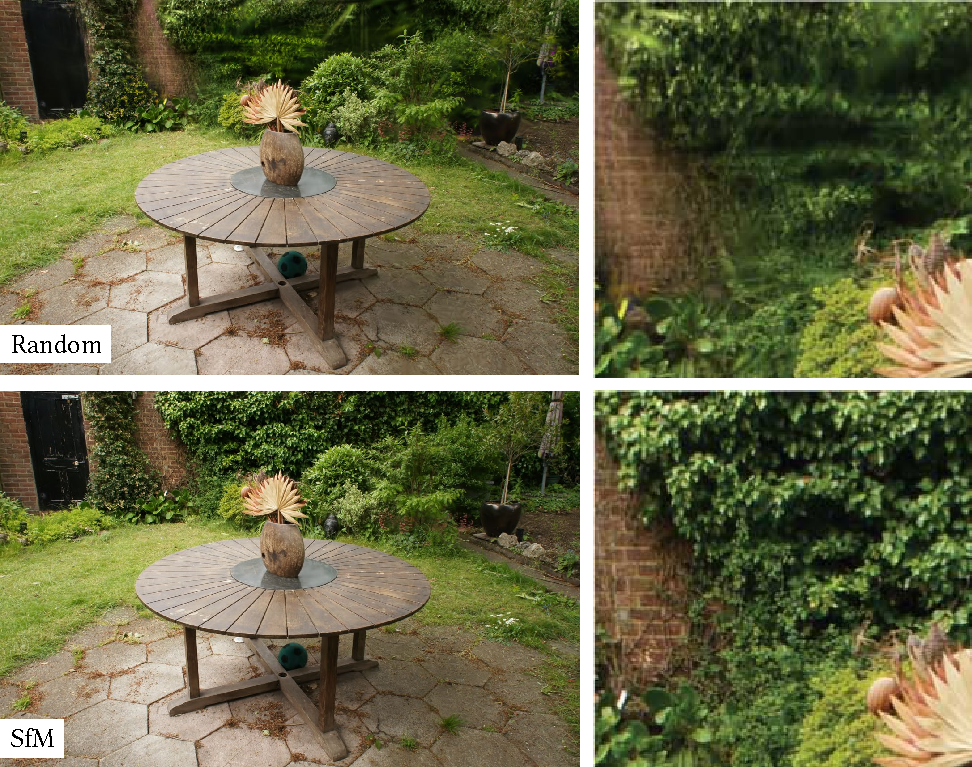
\includegraphics[width=\linewidth]{figures/ablations/random_vs_sfm2.pdf}
	\caption{
		\label{fig:random}
		Initialization with SfM points helps. Above: initialization with a random point cloud. Below: initialization using SfM points.
	}
\end{figure}

\paragraph{Initialization from SfM}
We also assess the importance of initializing the 3D Gaussians from the SfM point cloud. 
For this ablation, we uniformly sample a cube with a size equal to three times the extent of the input camera's bounding box. We observe that our method performs relatively well, avoiding complete failure even without the SfM points. Instead, it degrades mainly in the background, see Fig.~\ref{fig:random}. Also in areas not well covered from training views, the random initialization method appears to have more floaters that cannot be removed by optimization. On the other hand, the synthetic NeRF dataset does not have this behavior because it has no background and is well constrained by the input cameras (see discussion above).

\begin{figure}[!h]
	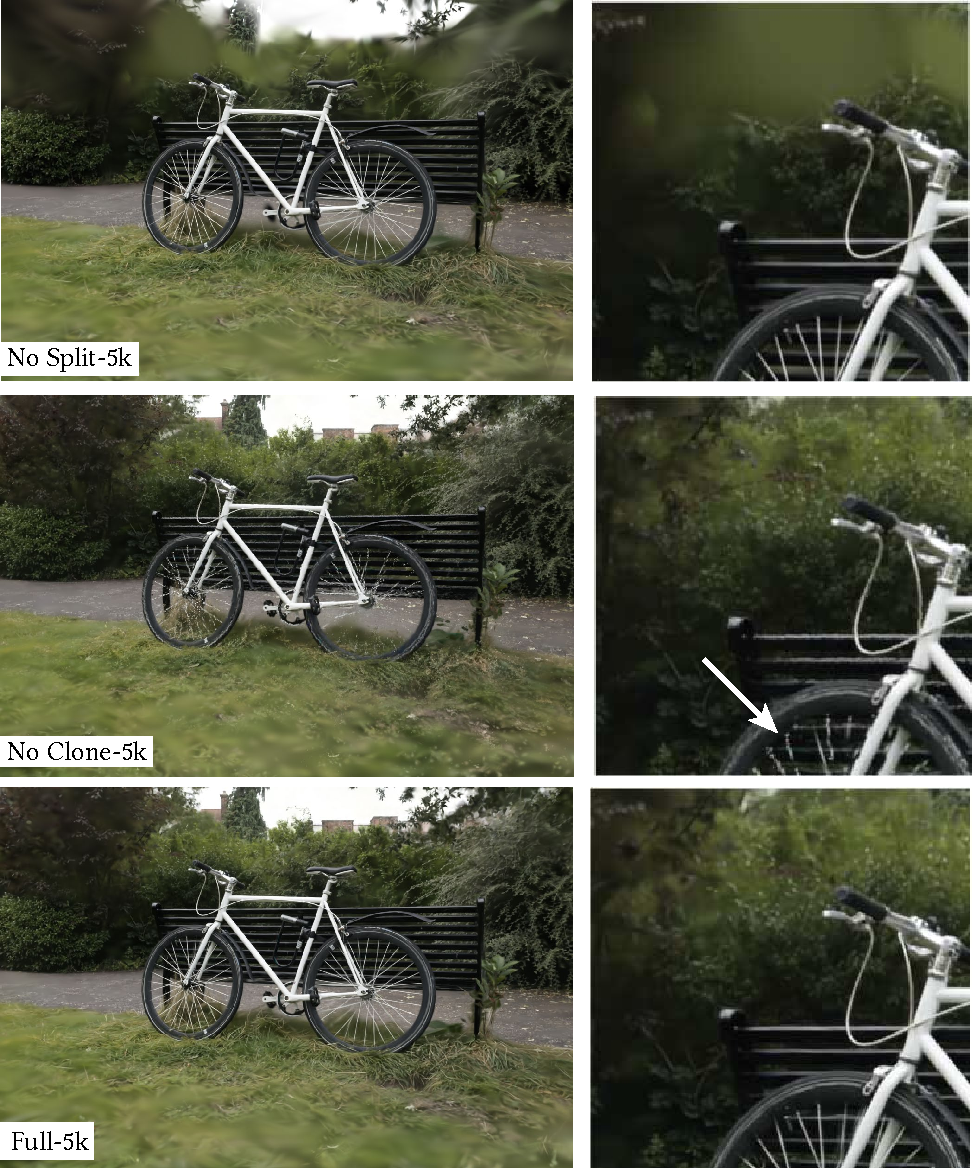
\includegraphics[width=\linewidth]{figures/ablations/densification.pdf}
	\caption{
		\label{fig:densification_ablate}
		Ablation of densification strategy for the two cases "clone" and "split" (Sec.~\ref{sec:opt-dens}).
	}
\end{figure}

\paragraph{Densification.}
We next evaluate our two densification methods, more specifically the clone and split strategy described in Sec.~\ref{sec:opt-dens}. We disable each method separately and optimize using the rest of the method unchanged. Results show that splitting big Gaussians is important to allow good reconstruction of the background as seen in Fig.~\ref{fig:densification_ablate}, while cloning the small Gaussians instead of splitting them allows for a better and faster convergence especially when thin structures appear in the scene. 

\begin{figure}[!h]
	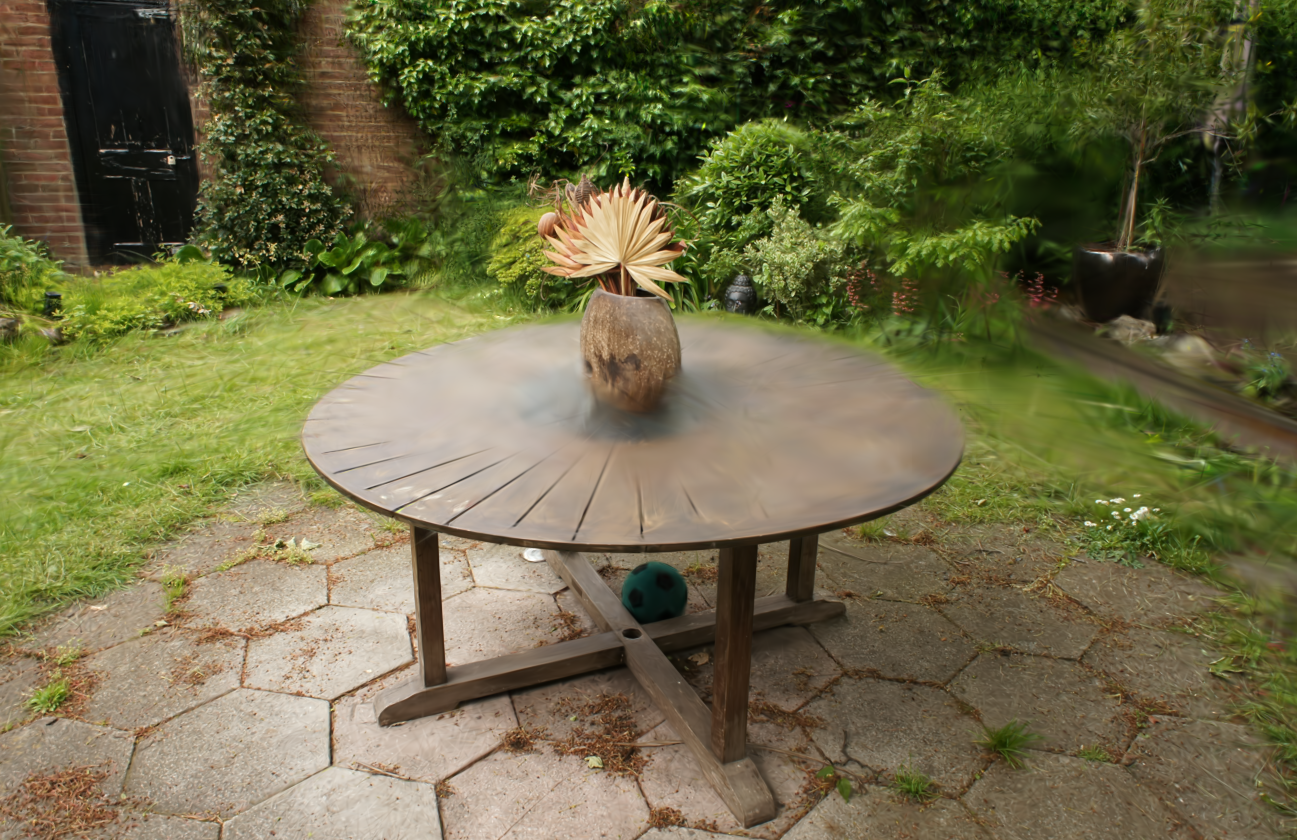
\includegraphics[width=.49\linewidth]{figures/ablations/images/30k/garden/limitedBW.png}
	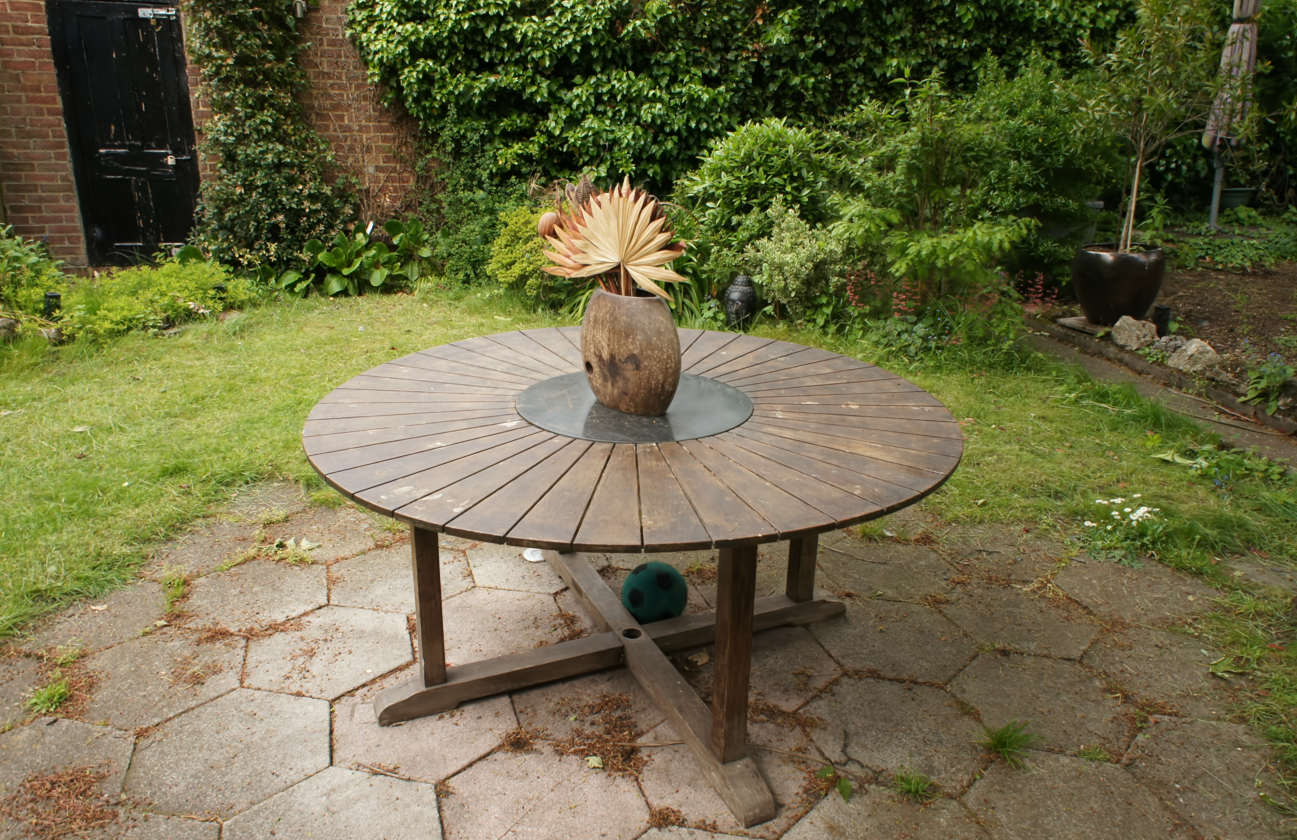
\includegraphics[width=.49\linewidth]{figures/ablations/images/30k/garden/full.png}
	\caption{
		If we limit the number of points that receive gradients, the effect on visual quality is significant.
		Left: limit of 10 Gaussians that receive gradients. Right: our full method.
		\label{fig:gradients}
	}
\end{figure}

\paragraph{Unlimited depth complexity of splats with gradients.}
We evaluate if skipping the gradient computation after the $N$ front-most points will give us speed without sacrificing quality, as suggested in ~Pulsar~\cite{Lassner_2021_CVPR}. In this test, we choose N=10, which is two times higher than the default value in ~Pulsar, but it led to unstable optimization because of the severe approximation in the gradient computation. For the \textsc{Truck} scene, quality degraded by 11dB in PSNR (see \CORRECTION{Tab.}{Table}~\ref{tab:ablation_table}, Limited-BW), and the visual outcome is shown in Fig.~\ref{fig:gradients} for \textsc{Garden}.





\paragraph{Anisotropic Covariance.}
An important algorithmic choice in our method is the optimization of the full covariance matrix for the 3D Gaussians. To demonstrate the effect of this choice, we perform an ablation where we remove anisotropy by optimizing a single scalar value that controls the radius of the 3D Gaussian on all three axes. The results of this optimization are presented visually in Fig.~\ref{fig:ablation-aniso}. We observe that the anisotropy significantly improves the quality of the 3D Gaussian's ability to align with surfaces, which in turn allows for much higher rendering quality while maintaining the same number of points.

\begin{figure*}[!h]
	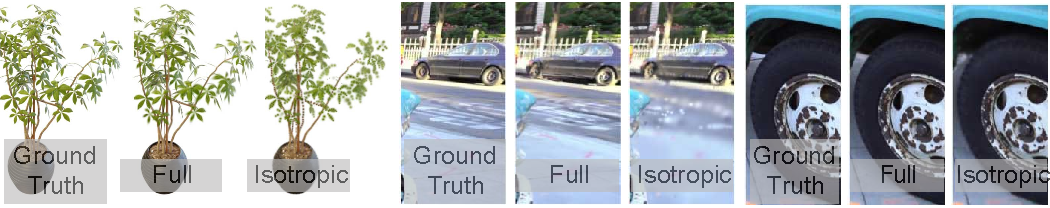
\includegraphics{figures/ablations/isotropy_vs_anisotropy2.pdf}
	\caption{
		\label{fig:ablation-aniso}
		We train scenes with Gaussian anisotropy disabled and enabled. The use of anisotropic volumetric splats enables modelling of fine structures and has a significant impact on visual quality. Note that for illustrative purposes, we restricted \textsc{Ficus} to use no more than 5k Gaussians in both configurations.
	}
\end{figure*}





\paragraph{Spherical Harmonics.}
Finally, the use of spherical harmonics improves our overall PSNR scores since they compensate for the view-dependent effects (\CORRECTION{Tab.}{Table}~\ref{tab:ablation_table}).




\subsection{Limitations}

Our method is not without limitations. 
In regions where the scene is not well observed we have artifacts; in such regions, other methods also struggle (e.g., Mip-NeRF360 in Fig.~\ref{fig:limit}). 
Even though the anisotropic Gaussians have many advantages as described above, 
our method can create elongated artifacts or ``splotchy'' Gaussians (see Fig.~\ref{fig:limit-under}); again previous methods also struggle in these cases.  

We also occasionally have popping artifacts when our optimization creates large Gaussians; this tends to happen in regions with view-dependent appearance. %
One reason for these popping artifacts is the trivial rejection of Gaussians via a guard band in the rasterizer. A more principled culling approach would alleviate these artifacts. \ADDITION{Another factor is our simple visibility algorithm, which can lead to Gaussians suddenly switching depth/blending order. This could be addressed by antialiasing, which we leave as future work.}
Also, we currently do not apply any regularization to our optimization; doing so would help with both the unseen region and popping artifacts. 

\ADDITION{While we used the same hyperparameters for our full evaluation, early experiments show that reducing the position learning rate can be necessary to converge in very large scenes (e.g., urban datasets).}

Even though we are very compact compared to previous point-based approaches, our memory consumption is significantly higher than NeRF-based solutions. \ADDITION{During training of large scenes, peak GPU memory consumption can exceed 20~GB in our unoptimized prototype. However, this figure could be significantly reduced by a careful low-level implementation of the optimization logic (similar to InstantNGP). Rendering the trained scene requires sufficient GPU memory to store the full model (several hundred megabytes for large-scale scenes) and an additional 30--500 MB for the rasterizer, depending on scene size and image resolution. We note that there are many opportunities to further reduce memory consumption of our method.} Compression techniques for point clouds is a well-studied field~\cite{de2016compression}; it would be interesting to see how such approaches could be adapted to our representation.



\begin{figure}[!h]
	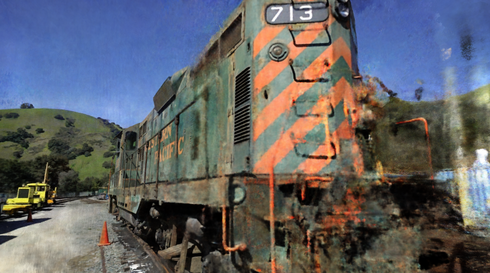
\includegraphics[width=0.49\columnwidth]{results/limitations/color_009_s.png}
	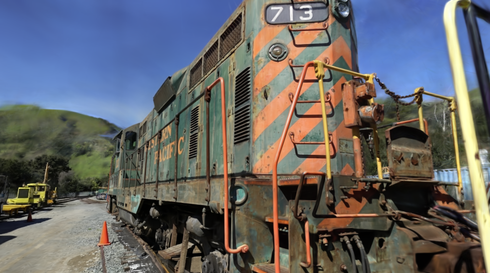
\includegraphics[width=0.49\columnwidth]{results/limitations/00073_s.png}
	\caption{
		\label{fig:limit}
		Comparison of failure artifacts: Mip-NeRF360 has ``floaters'' and grainy appearance (left, foreground), while our method produces coarse, anisoptropic Gaussians resulting in low-detail visuals (right, background). \textsc{Train} scene.
	}
\end{figure}

\begin{figure}[!h]
	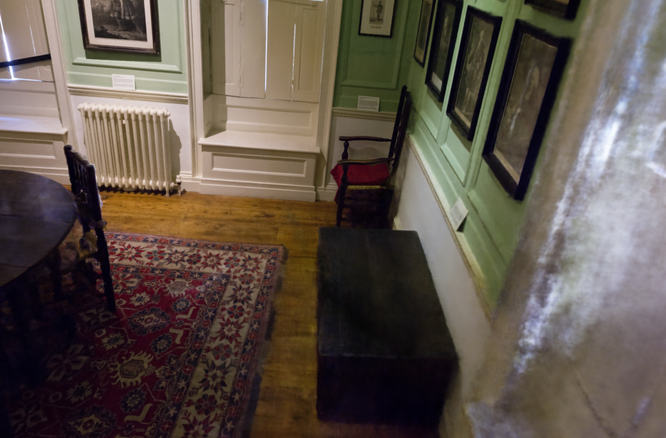
\includegraphics[width=0.49\linewidth]{figures/extremeviews/color_032_s.png}
	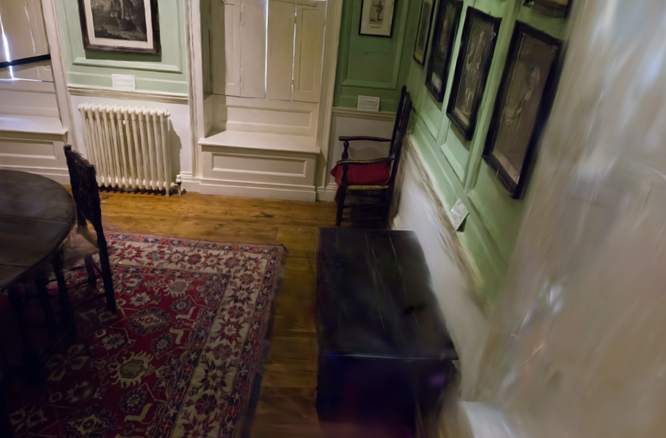
\includegraphics[width=0.49\linewidth]{figures/extremeviews/IMG_6589_s.png}
	\caption{
		In views that have little overlap with those seen during training, our method may produce artifacts (right). Again, Mip-NeRF360 also has artifacts in these cases (left). \textsc{DrJohnson} scene.
		\label{fig:limit-under}
	}
\end{figure}
